%%%%%%%%%%%%%%%%%%%%%%%%%%%%%%%%%%%%%
%                                   %
% Compile with XeLaTeX and biber    %
%                                   %
% Questions or comments:            %
%                                   %
% joshua dot mcneill at uga dot edu %
%                                   %
%%%%%%%%%%%%%%%%%%%%%%%%%%%%%%%%%%%%%

\documentclass{beamer}
  % Read in standard preamble (cosmetic stuff)
  %%%%%%%%%%%%%%%%%%%%%%%%%%%%%%%%%%%%%%%%%%%%%%%%%%%%%%%%%%%%%%%%
% This is a standard preamble used in for all slide documents. %
% It basically contains cosmetic settings.                     %
%                                                              %
% Joshua McNeill                                               %
% joshua dot mcneill at uga dot edu                            %
%%%%%%%%%%%%%%%%%%%%%%%%%%%%%%%%%%%%%%%%%%%%%%%%%%%%%%%%%%%%%%%%

% Beamer settings
% \usetheme{Berkeley}
\usetheme{CambridgeUS}
% \usecolortheme{dove}
% \usecolortheme{rose}
\usecolortheme{seagull}
\usefonttheme{professionalfonts}
\usefonttheme{serif}
\setbeamertemplate{bibliography item}{}

% Packages and settings
\usepackage{fontspec}
  \setmainfont{Charis SIL}
\usepackage{hyperref}
  \hypersetup{colorlinks=true,
              allcolors=blue}
\usepackage{graphicx}
  \graphicspath{{../../figures/}}
\usepackage[normalem]{ulem}
\usepackage{enumerate}

% Document information
\author{M. McNeill}
\title[FREN2001]{Français 2001}
\institute{\url{joshua.mcneill@uga.edu}}
\date{}

%% Custom commands
% Lexical items
\newcommand{\lexi}[1]{\textit{#1}}
% Gloss
\newcommand{\gloss}[1]{`#1'}
\newcommand{\tinygloss}[1]{{\tiny`#1'}}
% Orthographic representations
\newcommand{\orth}[1]{$\langle$#1$\rangle$}
% Utterances (pragmatics)
\newcommand{\uttr}[1]{`#1'}
% Sentences (pragmatics)
\newcommand{\sent}[1]{\textit{#1}}
% Base dir for definitions
\newcommand{\defs}{../definitions}


  % Packages and settings

  % Document information
  \subtitle[Nationalités et \lexi{venir}]{Les nationalités et le verbe \lexi{venir}}

\begin{document}
  % Read in the standard intro slides (title page and table of contents)
  \begin{frame}
    \titlepage
    \tiny{Office: % Basically a variable for office hours location
Gilbert 121\\
          Office hours: % Basically a variable for office hours
 lundi, mercredi, vendredi 10:10--11:10
}
  \end{frame}

  \begin{frame}{}
    \begin{center}
      \begin{tabular}{l | l l | l l}
  \multicolumn{5}{c}{venir \gloss{to come}} \\
  \hline
      & \multicolumn{2}{l |}{singulier} & \multicolumn{2}{l}{pluriel} \\
  \hline
  1re & je         & viens              & nous        & venons \\
  2e  & tu         & viens              & vous        & venez \\
  \hline
  3e  & il (masc)  &                    & ils (masc)  & \\
      & elle (fem) & vient              & elles (fem) & viennent \\
      & on         &                    &             & \\
  \hline
  \multicolumn{5}{c}{Impératifs $\to$ viens, venez, venons} \\
  \multicolumn{5}{c}{Passé composé $\to$ je suis venu/e} \\
  \multicolumn{5}{c}{Futur simple $\to$ je viendrai}
\end{tabular}

    \end{center}
  \end{frame}

  \begin{frame}{Nationalités}
    \footnotesize
    \begin{columns}
      \column{0.5\textwidth}
        D'où vient cette personne, et quelle est sa nationalité?
        \only<1-4>{
          \begin{enumerate}
            \item Mon pays est en Afrique. Presque tous mes amis sont musulmans. Nous parlons arabe mais ceux qui sont allés à l'université parlent français, aussi. Nous sommes à côté de l'océan Atlantique, mais nous avons également un grand désert.
            \item<2->[$\to$] Il/Elle vient du Maroc. Il/Elle est marocain/e.
            \item<3-> Dans le passé, nos leaders parlaient français, même si mon pays est en Asie. Il y a des jungles dans mon pays, et on cultive beaucoup de riz grâce aux moussons \gloss{monsoons}.
            \item<4->[$\to$] Il/Elle vient du Vietnam. Il/Elle est vietnamien/ne.
          \end{enumerate}
        }
        \only<5-8>{
          \begin{enumerate}
            \setcounter{enumi}{2}
            \item<5-> Quelquefois, les Américains nous confondent avec les Australiens, mais mon pays est une île beaucoup plus petite que l'Australie, toujours dans l'océan Pacifique. Peut-être que vous connaissez l'un des films tourné ici: Le Seigneur des anneaux.
            \item<6->[$\to$] Il/Elle vient de Nouvelle-Zélande. Il/Elle est néo-zélandais/e.
            \item<7-> Mon pays est compliqué, surtout notre rapport avec les États-Unis. Nous sommes actuellement en guerre avec l'Ukraine.
            \item<8->[$\to$] Il/Elle vient de Russie. Il/Elle est russe.
          \end{enumerate}
        }
      \column{0.5\textwidth}
        \begin{minipage}[c][0.8\textheight]{\linewidth}
          \begin{center}
            \only<1-2>{
              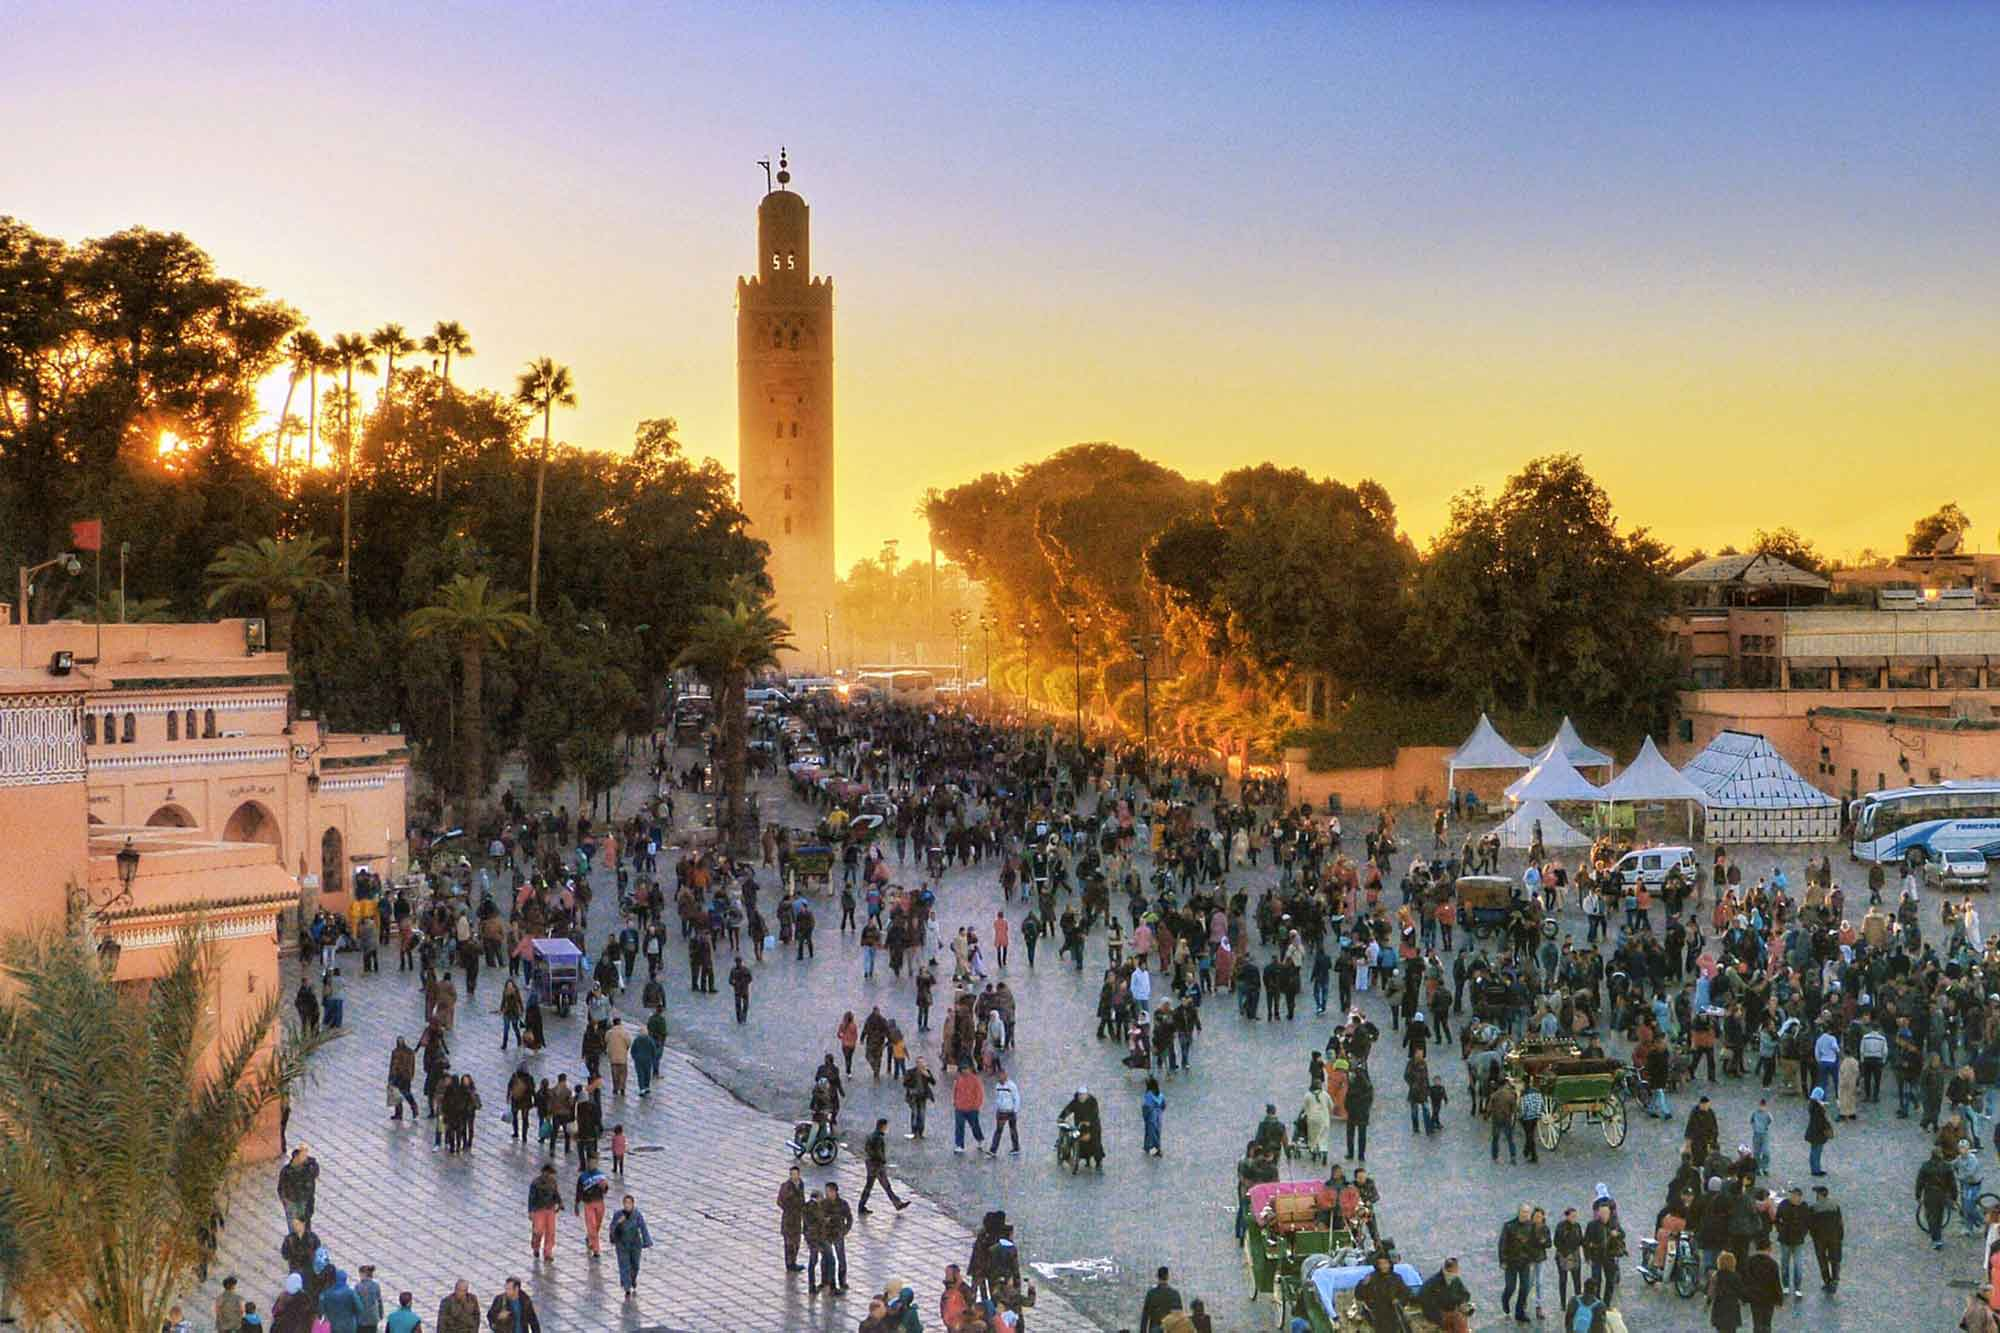
\includegraphics[scale=0.085]{maroc.jpg}
            }
            \only<3-4>{
              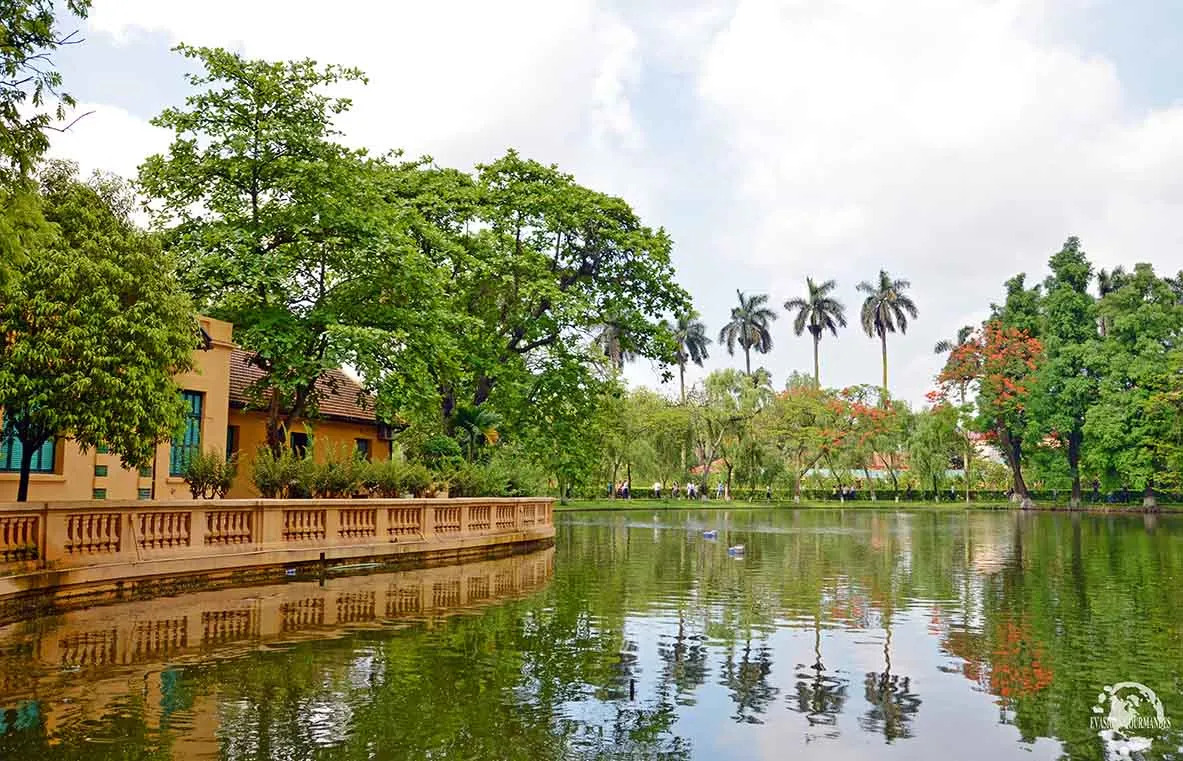
\includegraphics[scale=0.145]{vietnam.jpg}
            }
            \only<5-6>{
              \includegraphics[scale=0.145]{nouvelle-zélande.jpg}
            }
            \only<7-8>{
              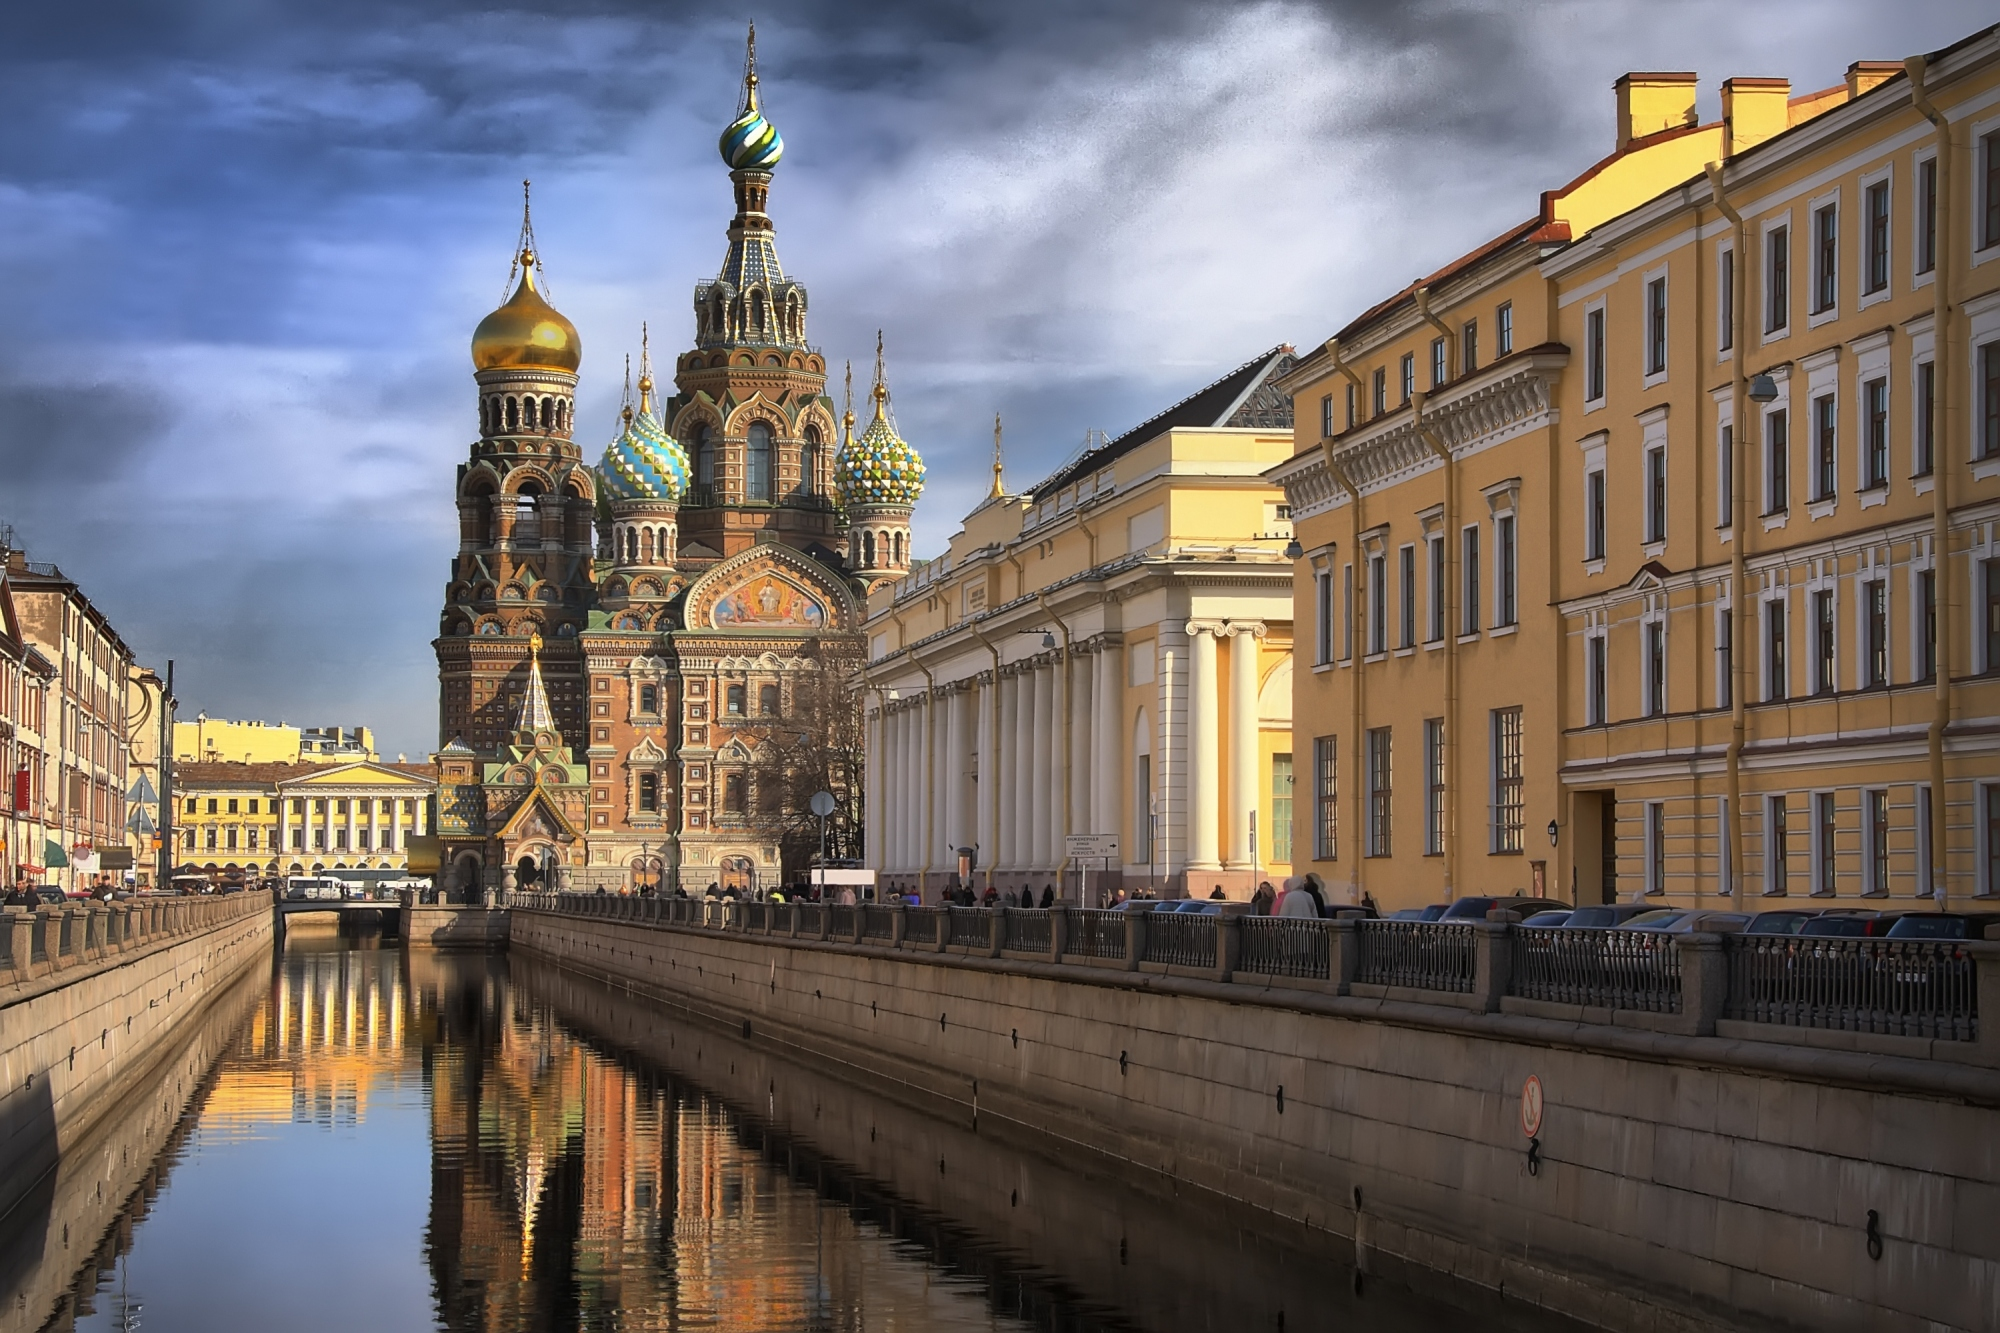
\includegraphics[scale=0.085]{russie.jpg}
            }
          \end{center}
        \end{minipage}
    \end{columns}
  \end{frame}

  \begin{frame}{}
    \begin{center}
      \Large Quiz
    \end{center}
  \end{frame}

  \begin{frame}{Vos origines}
    En groupes de 3 ou 4, \alert{discutez} d'où viennent vos ancêtres \gloss{ancestors}.
    Commment sont ces pays ou ces villes?
    \begin{description}
      \item[] \textbf{Modèle:}
      \item[E1:] Où viennent tes ancêtres?
      \item[E2:] Ma grand-mère est née à Shanghai en Chine. Je ne l'ai jamais visité, mais elle me dit qu'il y a beaucoup de gens. Et vous?
      \item[E3:] Moi, j'ai des ancêtres d'Haïti. J'y suis allée une fois. C'est un pays pauvre, mais la culture est riche.
      \item[E1:] Mes ancêtres viennent d'ici. Ils étaient des Amérindiens, spécifiquement des Cherokees de Géorgie.
    \end{description}
  \end{frame}

  \begin{frame}{}
    \begin{center}
      \Large Questions?
    \end{center}
  \end{frame}
\end{document}
